%
% relazione_es6.tex
%
% Copyright (C) 2016 frnmst (Franco Masotti) <franco.masotti@student.unife.it>
%                    dannylessio (Danny Lessio)
%
% This file is part of networks-lab.
%
% networks-lab is free software: you can redistribute it and/or modify
% it under the terms of the GNU General Public License as published by
% the Free Software Foundation, either version 3 of the License, or
% (at your option) any later version.
%
% networks-lab is distributed in the hope that it will be useful,
% but WITHOUT ANY WARRANTY; without even the implied warranty of
% MERCHANTABILITY or FITNESS FOR A PARTICULAR PURPOSE.  See the
% GNU General Public License for more details.
%
% You should have received a copy of the GNU General Public License
% along with networks-lab.  If not, see <http://www.gnu.org/licenses/>.
%


\makeatletter
\def\blfootnote{\xdef\@thefnmark{}\@footnotetext}
\makeatother

\documentclass[9pt, a4paper, oneside]{article}
\usepackage[a4paper]{geometry}
\usepackage{graphicx} % pictures
\usepackage{float} % used for H option in pictures                        
\usepackage{setspace} % packets
\usepackage{listings}
\singlespacing % interlinea singolo
\title{Relazione esercitazione 7 Laboratorio di reti\newline
Invio e ricezione di email tra varie reti}
\author{Franco Masotti \and Danny Lessio}
\date{May 25, 2015}
\begin{document}
	\maketitle
	\tableofcontents
	\newpage
    \footnotetext{networks-lab  Copyright (C) 2016  frnmst (Franco Masotti)$
dannylessio (Danny Lessio).  This document comes with ABSOLUTELY NO WARRANT$
This is free software, and you are welcome to redistribute it
under certain conditions; see LICENSE file for details.}
	\part{Consegna}
			\par
				Lo scopo dell'esercitazione \'e quello di 
				inviare e ricevere mail tra tutti i gruppi che 
				sono connessi ai rispettivi router. Usando uno 
				schema simile al precedente per le 
				connessioni seriali bisogna configurare i 
				server DNS in modo che qualunque nome host 
				appartenente ad un gruppo possa essere 
				risolto. 
			\par
				Di seguito \'e rappresentato il nuovo schema 
				dei collegamenti tra le seriali di tutti i router:
				\begin{figure}[H]
					\centering
					\caption{Nuove connessioni}
					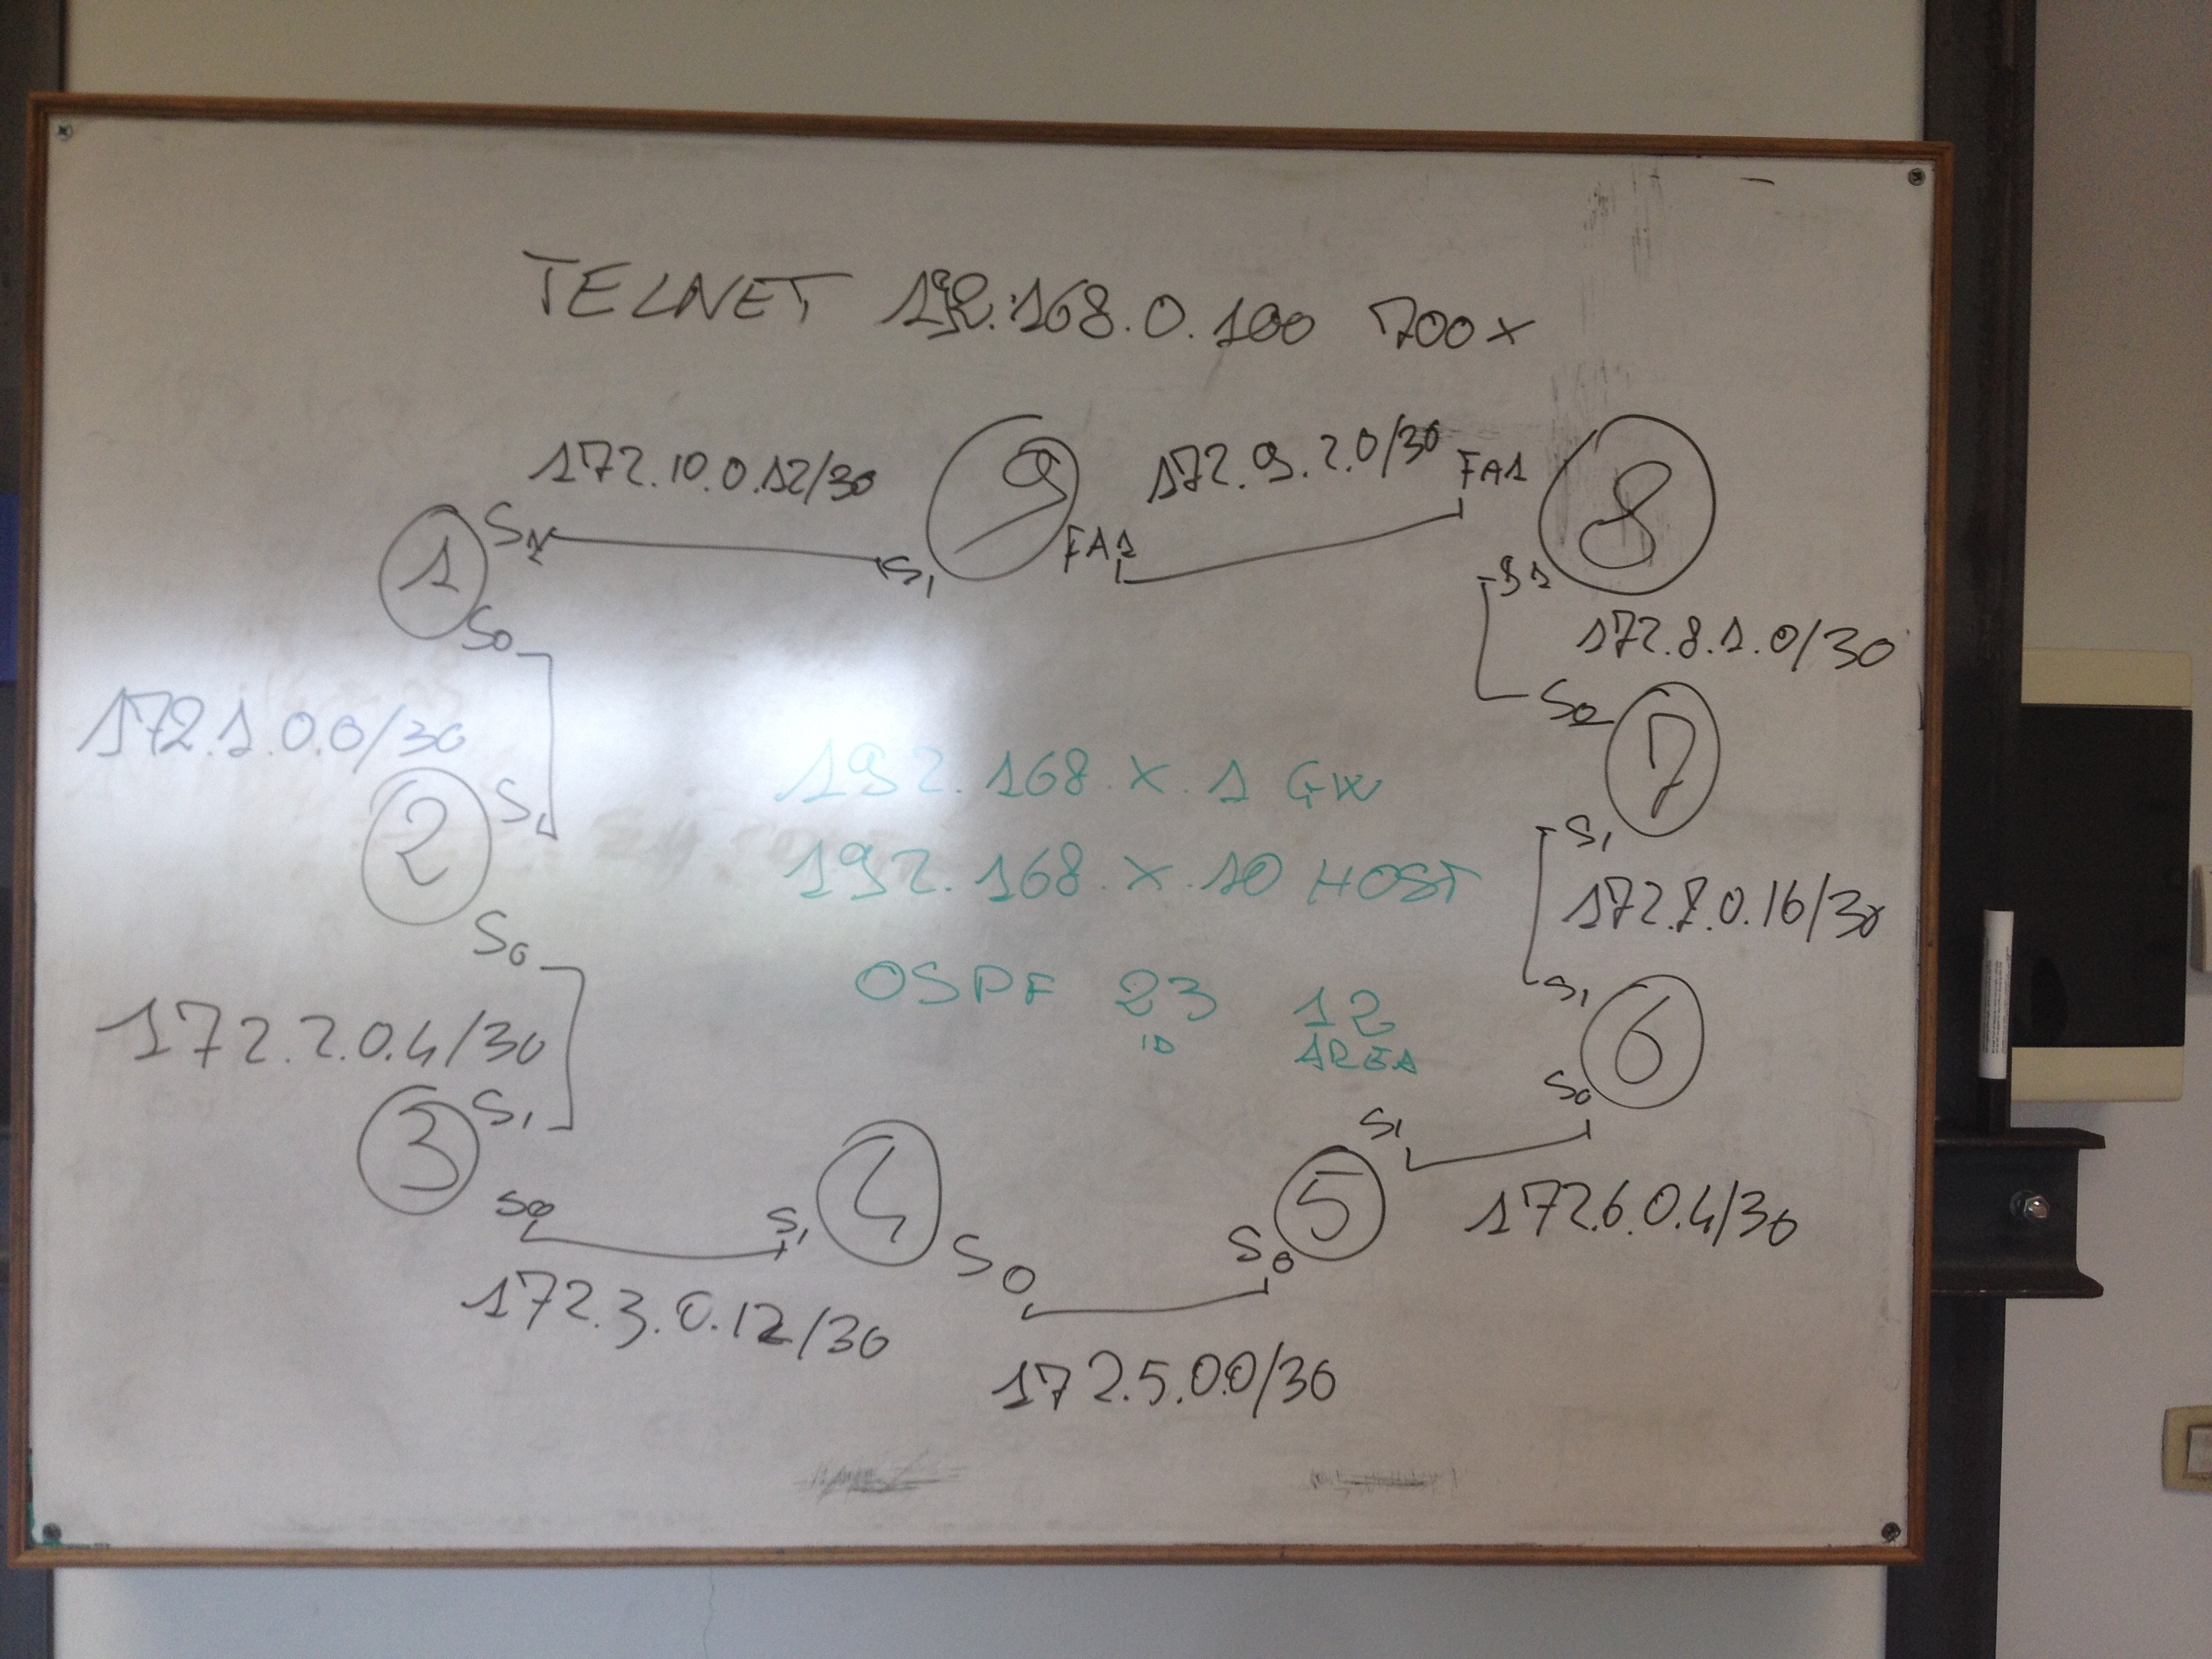
\includegraphics[scale=0.12]{../source/schema_connessioni.jpg}
				\end{figure}
		\newpage
	\part{Configurazione del router}
		\section{Modifica delle seriali}
			\par
				Rispetto all'esercitazione precedente \'e 
				cambiata una porta seriale. Adesso abbiamo 
				una porta di tipo DCE e l'altra di tipo DTE. 
				Per questo motivo abbiamo dovuto settare clock 
				rate sulla porta DCE.
				\begin{verbatim}
enable
configure terminal
interface Serial0/1
clock rate 56000
				\end{verbatim}
		\section{OSPF}
			\par
				Affinch\'e i router ed i computer possano  
				comunicare tra di loro, abbiamo usato 
				\texttt{OSPF} come protocollo di routing. \'E 
				stato sufficiente modificare il file 
				\texttt{running-config} con le 
				nuove informazioni di \texttt{OSPF} per ogni 
				interfaccia:
				\begin{verbatim}
ospf 23 area 12
				\end{verbatim}
		\section{Altre modifiche}
			\par
				L'indirizzo del nostro router deve essere 
				\texttt{192.168.2.1/24}, quindi abbiamo 
				modificato la entry in questo modo:
				\begin{verbatim}
ip address 192.168.2.1 255.255.255.0
				\end{verbatim}
			\par
				Dopo aver fatto queste modifiche 
				direttamente al file, abbiamo abilitato 
				l'ethernet sul router ed abbiamo caricato il 
				file stesso con tftp.
		\section{IPv6}
			\par
				In questa esercitazione abbiamo abilitato anche 
				l'IPv6 sul router usando i seguenti indirizzi:
				\begin{itemize}
					\item
						L'indirizzo 
						dell'ethernet \'e 
						\texttt{2002::1/64}
					\item
						L'indirizzo della seriale 0 \'e 
						\texttt{1002::5/127}
					\item
						L'indirizzo della seriale 1 \'e 
						\texttt{1001::1/127}
				\end{itemize}
				Per assegnare gli indirizzi IPv6:
				\begin{verbatim}
enable
configure terminal
interface <interface>
ipv6 address <address>
ipv6 enable
				\end{verbatim}
				OSPF va abilitato anche per IPv6. Per ogni 
				interfaccia abbiamo dato il seguente comando:
				\begin{verbatim}
ipv6 ospf 23 area 12				
				\end{verbatim}
		\newpage
	\part{Configurazione del computer}
		\section{Default gateway}
			\par
				Per fare in modo che i nostri server fossero 
				raggiunti dalle macchine delle altre sottoreti
				abbiamo settato il nostro router come default 
				gateway\footnote{Per qualche motivo questo 
				comando non funziona sempre. Assegnandolo con 
				il network manager questo problema non si 
				pone.}:
				\begin{verbatim}
sudo ip route add default via 192.168.2.1
				\end{verbatim}
		\section{File di configurazione dei server DNS root}
			\par
				\'E necessario dover configurare un file di 
				che gestisce i server DNS master all'interno 
				di \texttt{BIND} per poter comunicare con gli 
				altri gruppi. Infatti se il nostro server DNS 
				non conosce gli instradamenti relativi alla 
				propria sottorete interrogher\'a i server 
				descritti all'interno di questo file.
			\par	
				Per prima cosa \'e necessario dover modificare 
				il file \texttt{named.conf} aggiungendo queste 
				righe:
				\begin{verbatim}
zone "." {
  type hint;
  file "root.hint";
};
				\end{verbatim}				
				Abbiamo definito 
				\texttt{root.hint}\footnote{Vedi sezione 
				listati} come file contentente le entry dei 
				server DNS di root. Successivamente lo 
				abbiamo aggiornato con i name server 
				relativi agli altri 8 gruppi escluso il 
				nostro\footnote{Lo scheletro del file \'e stato 
				reperito da 
				https://www.iana.org/domains/root/files}. 
			\par
				Per poter vedere se gli altri server sono a 
				noi raggiungibili possiamo lanciare il comando 
				\texttt{show ip route}, che ci mostrer\'a lo 
				stato corrente della tabella di routing.
				Lanciando il comando \texttt{dig -x} con il 
				nome di un server DNS di un altro gruppo  
				\footnote{Tipicamente \'e \texttt{ns}}, 
				possiamo verificarne la risposta:
				\begin{verbatim}
dig -x ns.gruppox.labreti.it
				\end{verbatim}
		\section{Mail}
			\par
				A questo punto siamo tornati all'esercitazione 
				4 ed abbiamo avviato tutti i programmi 
				necessari per l'invio e ricezione delle mail. 
				Tuttavia per inviare mail \'e stato necessario 
				modificare il file \texttt{master.cf} di 
				Postfix. Avevamo infatti aggiunto restrizioni 
				per quanto riguarda i mittenti ed i 
				destinatari. Abbiamo verificato che \'e stato 
				possibile inviare le email agli altri gruppi 
				grazie a Sylpheed.
			\par
				Per mancanza di tempo non siamo riusciti a 
				ricevere le mail sempre a causa di 
				impostazioni di sicurezza nella quinta 
				esercitazione. Sarebbe stato necessario pi\'u 
				tempo per riguradare attentamente tutte le 
				opzioni nel file \texttt{master.cf} di Postfix.
		\newpage
	\part{Listati}	
		 \par		
		 \section{\texttt{running-config} OSPF IPv6}
			\par
				\texttt{running-config}
			\par
				File di configurazione principale del router 
				configurato per il routing OSPF e l'IPv6.
			\texttt{\lstinputlisting[breaklines]{../source/running-config-ospf-ipv6}}
			\newpage
		\section{\texttt{root.hint} BIND}
			\par
			 	\texttt{root.hint}
			\par
				File di configurazione nel quale vengono 
				elencati i DNS master server (in questo caso 
				vengono definiti anche i server DNS degli 
				altri 8 gruppi, infatti l'unico server non 
				presente \'e il nostro). 	
			\texttt{\lstinputlisting[breaklines]{../source/root.hint}}
\end{document}

